\section{Business Process Model and Notation (BPMN)}

\subsection{BPMN Syntax}
BPMN is a graphical representation for specifying business processes in a business process model. It provides a standard notation that is readily understandable by all business stakeholders, including business analysts, technical developers, and business managers.

\subsubsection{Core Elements}
The core elements of BPMN can be categorized into four main groups:
\begin{figure}[H]
    \centering
    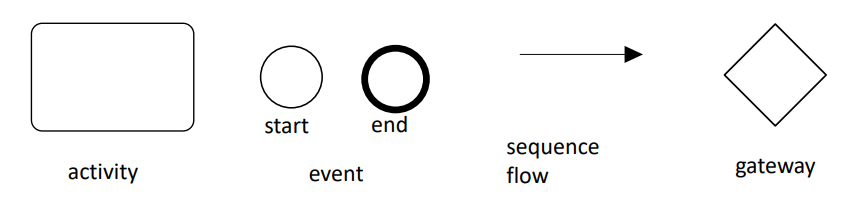
\includegraphics[width=0.8\textwidth]{images/bpmn/core.png}
    \caption{Core Elements of BPMN}
\end{figure}
\begin{enumerate}
    \item \textbf{Events}: represent something that happens during the course of a business process. The core types of events are:
    \begin{itemize}
        \item \textbf{Start Event}: trigger a new process instance, by generating a token to start the process;
        \item \textbf{End Event}: signals that a process instance has completed its execution, by consuming a token.
    \end{itemize}
    \item \textbf{Gateways}: represent decision points in a process where the flow can diverge or converge based on certain conditions. The core types of gateways are:
    \begin{itemize}
        \item \textbf{XOR Gateway (Exclusive Gateway)}: represents a decision point where only one of the outgoing paths can be taken based on conditions. The \textbf{XOR-split} takes one
        outgoing branch, while the \textbf{XOR-join} proceeds when one incoming branch completes. 
        \begin{figure}[H]
            \centering
            \begin{minipage}[t]{0.25\textwidth}
                \centering
                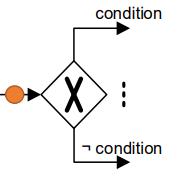
\includegraphics[width=\linewidth]{images/bpmn/XORsplit.png}
            \end{minipage}\hfill
            \begin{minipage}[t]{0.25\textwidth}
                \centering
                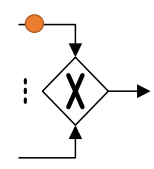
\includegraphics[width=\linewidth]{images/bpmn/XORjoin.png}
            \end{minipage}\hfill
            \caption{XOR-split and XOR-join Gateways}
        \end{figure}
        \item \textbf{AND Gateway (Parallel Gateway)}: provides a mechanisms to create and synchronize parallel paths in the process flow.
        The \textbf{AND-split} creates multiple concurrent paths (all outgoing branches are taken), while the \textbf{AND-join} synchronizes multiple incoming paths (waits for all incoming branches to complete before proceeding).
        \begin{figure}[H]
            \centering
            \begin{minipage}[t]{0.25\textwidth}
                \centering
                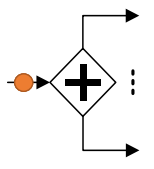
\includegraphics[width=\linewidth]{images/bpmn/ANDsplit.png}
            \end{minipage}\hfill
            \begin{minipage}[t]{0.25\textwidth}
                \centering
                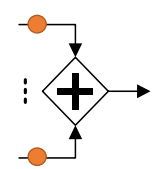
\includegraphics[width=\linewidth]{images/bpmn/ANDjoin.png}
            \end{minipage}
            \caption{AND-split and AND-join Gateways}
        \end{figure}
        \item \textbf{OR Gateway}: provide a mechanism to create and synchronize $m$ out of $n$ paths in the process flow.
        The \textbf{OR-split} can take one or more outgoing branches, while the \textbf{OR-join} waits for all the active incoming branches to complete before proceeding.
        \begin{figure}[H]
            \centering
            \begin{minipage}[t]{0.25\textwidth}
                \centering
                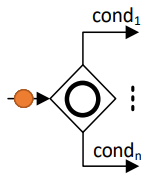
\includegraphics[width=\linewidth]{images/bpmn/ORsplit.png}
            \end{minipage}\hfill
            \begin{minipage}[t]{0.25\textwidth}
                \centering
                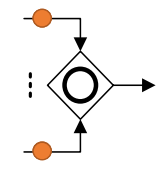
\includegraphics[width=\linewidth]{images/bpmn/ORjoin.png}
            \end{minipage}
            \caption{OR-split and OR-join Gateways}
        \end{figure}
    \end{itemize}
\end{enumerate}
\subsubsection{Naming conventions} 
It is important to follow naming conventions for clarity:
\begin{itemize}
    \item \textbf{Event}: Use noun + past participle (e.g., "Order Received").
    \item \textbf{Activity}: Use verb + noun (e.g., "Approve Invoice").
    \item \textbf{Split Gateway}: Use descriptive labels with conditions(e.g., "Is Payment Approved?").
\end{itemize}

\subsubsection{Data Objects}
A \textbf{Data Object} captures an artifact required (input) or produced (output) by activities within a process. 
Can be physical (e.g., paper document) or digital (e.g., electronic file). You can also denote the \textbf{status} of the business object inside square brackets (e.g., [approved], [pending]).
\\\\An \textbf{association link} (dashed line) is used to connect data objects to activities or events of business processes.
All occurrences of a Data Object represent the same underlying data.
\\\\\textbf{Input data objects} represent a blocking condition for the activity to start (the activity cannot start until the input data object is available).
\begin{figure}[H]
    \centering
    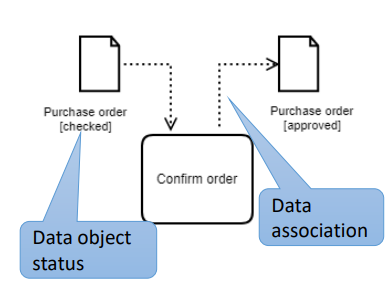
\includegraphics[width=0.4\textwidth]{images/bpmn/dataObject.png}
    \caption{Data Object in BPMN}
\end{figure}

\subsubsection{Data Store}
A Data Store is a place containing data objects that is persistent beyond the lifetime of a process instance. 
\begin{figure}[H]
    \centering
    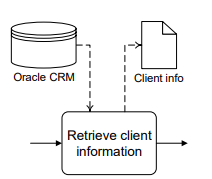
\includegraphics[width=0.4\textwidth]{images/bpmn/dataStore.png}
    \caption{Data Store in BPMN}
\end{figure}

\subsubsection{Text Annotations}\label{bpmn:textannotation}
A Text Annotation is used to add descriptive information to a BPMN diagram. It provides additional context or explanations about specific elements or the overall process flow.
Doesn't affect the process flow.
\begin{figure}[H]   
    \centering
    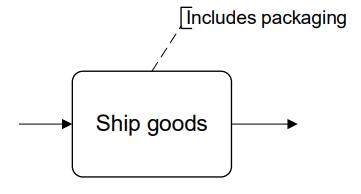
\includegraphics[width=0.4\textwidth]{images/bpmn/textAnnotation.png}
    \caption{Text Annotation in BPMN}
\end{figure}

\subsubsection{Pools and Lanes}
\textbf{Pools} captures a resource class. Generally used to model a business party (e.g., a whole company, department, or system).
\\\\\textbf{Lanes} are subdivisions within a pool that represent specific roles, departments, or functions within the business party. 
\begin{figure}[H]
    \centering
    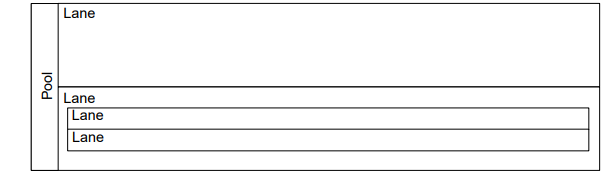
\includegraphics[width=0.6\textwidth]{images/bpmn/poolLane.png}
    \caption{Pools and Lanes in BPMN}
\end{figure}
Activity placed within a lane indicates that it is performed by the role or department represented by that lane.

\subsubsection{Message Flow} 
A Message Flow represents the flow of messages between two separate process participants (pools).
It indicates communication or interaction between different entities in a business process.
A Message Flow can connect:
\begin{itemize}
    \item directly the boundary of a pool (from a party to another party)
    \item to a specific activity or event within a pool (from a party to an activity/event or vice versa)
\end{itemize}
\begin{figure}[H]
    \centering
    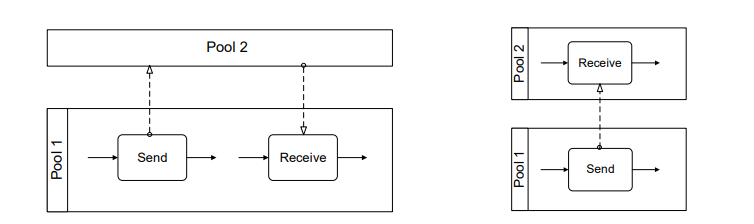
\includegraphics[width=0.6\textwidth]{images/bpmn/messageFlow.png}
    \caption{Message Flow in BPMN}
\end{figure}
These elements have some syntactic rules:
\begin{itemize}
    \item A \textbf{sequence flow} (solid line) cannot cross pool boundaries; it can only connect elements within the same pool;
    \item Both \textbf{sequence} and \textbf{message flows} can cross the boundaries of lanes within a pool;
    \item A \textbf{message flow} cannot connect two flow elements within the same pool;
\end{itemize}
An \textbf{incoming message flow} may lead to the creation of the data object by the activity receiving the message.

\subsection{Advanced BPMN Constructs}

\subsubsection{Sub-processes}
In BPMN, a sub-process is a compound activity that encapsulates a set of related tasks or activities within a larger process. 
It \textbf{requires} a \textbf{start event} and an end \textbf{event to define} its boundaries.
\begin{figure}[H]
    \centering
    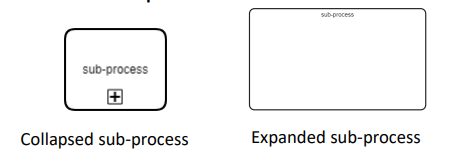
\includegraphics[width=0.6\textwidth]{images/bpmn/subprocess.png}
    \caption{Sub-process in BPMN}
\end{figure}
It can also delimit parts of the process that can be repeated or interrupted as a whole.

\subsubsection{Block-structured repetition}
Activity loop markers can be used to denote that an activity or sub-process can be repeated multiple times, based on certain conditions.
It can be used when we have a single entry and a single exit point for the repeated section of the process.
Then the completion condition is explicitly defined with a \textbf{textual annotation} (\ref{bpmn:textannotation}).
\begin{figure}[H]
    \centering
    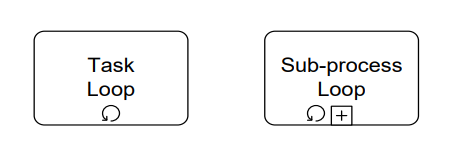
\includegraphics[width=0.4\textwidth]{images/bpmn/activityloop.png}
    \caption{Activity Loop Marker in BPMN}
\end{figure}    

\subsubsection{Parallel repetition: multi instance activity}
The multi-instance marker indicates that an activity or sub-process can be executed multiple times concurrently.
Useful when the same activity need to be performed for multiple instances of a data object (e.g., processing multiple orders).
\begin{figure}[H]
    \centering
    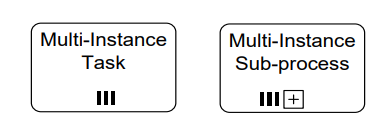
\includegraphics[width=0.4\textwidth]{images/bpmn/multiinstance.png}
    \caption{Multi-instance Marker in BPMN}
\end{figure}
We can also use a textual annotation to specify the number of instances or the conditions for creating new instances.
Then we can use this notation also for pools and lanes to indicate that multiple instances of a resource class are involved in the process.

\subsubsection{Events}
Events in BPMN represent something instantaneous that happens during the execution of a process. They are classified as follows:
\begin{figure}[H]
    \centering
    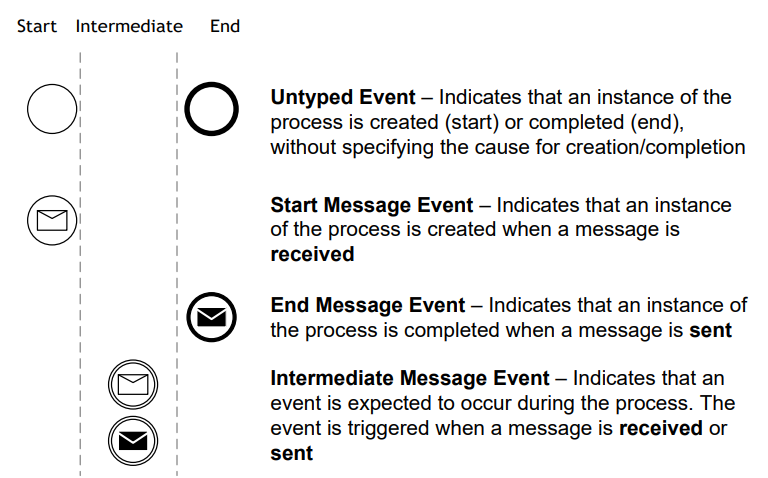
\includegraphics[width=0.8\textwidth]{images/bpmn/eventtable1.png}
\end{figure}
\begin{figure}[H]
    \centering
    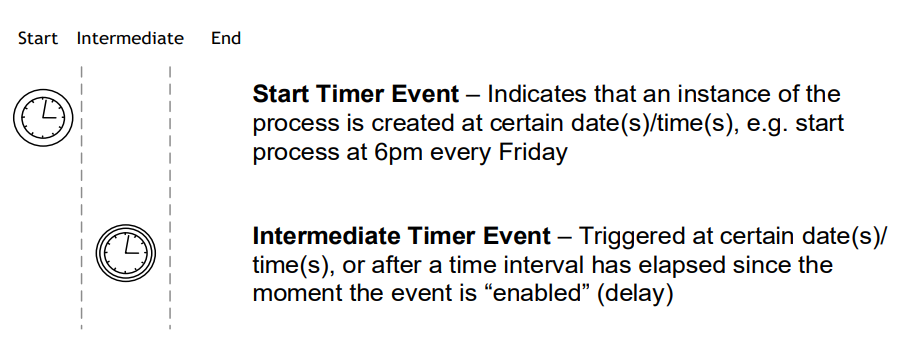
\includegraphics[width=0.8\textwidth]{images/bpmn/eventtable2.png}
\end{figure}

\paragraph{Untyped events:} they are the default events (start and end), already introduced in the core elements.
\paragraph{Message events:} represent the sending or receiving of a message between two process participants (pools).
\begin{itemize}
    \item \textbf{Message Start Event}: triggers a new process instance upon receiving a message;
    \item \textbf{Message End Event}: indicates that a message is sent when the process instance completes;
    \item \textbf{Message Intermediate:} can be used to send (black envelope) or receive (white envelope) messages during the execution of a process instance.
\end{itemize}
It's important to use message events only when the corresponding activity would simply send or receive a message without any additional processing.
Message receive events should be used to model the receipt of messages that trigger the start of a process or an intermediate event within a process, and not to model the receipt of messages that are part of the normal flow of activities within a process.
\paragraph{Temporal events:} represent time-based triggers or delays within a process.
\begin{itemize}
    \item \textbf{Timer Start Event}: triggers a new process instance based on a specific time or date;
    \item \textbf{Timer Intermediate Event}: can be used to introduce delays or wait for a specific time during the execution of a process instance.
\end{itemize}

\paragraph{Event-based decision}
Sometimes, a decision point in a process is based on the occurrence of specific events rather than conditions evaluated on data. In such cases, an event-based gateway is used to model the decision point.
It works similarly to an XOR gateway, but instead of evaluating conditions on data, it waits for one of the specified events to occur before proceeding along the corresponding path.
\begin{figure}[H]
    \centering
    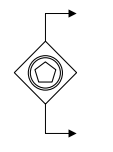
\includegraphics[width=0.2\textwidth]{images/bpmn/eventbasedxor.png}
    \caption{Event-based Gateway in BPMN}
\end{figure}
\begin{figure}[H]   
    \centering
    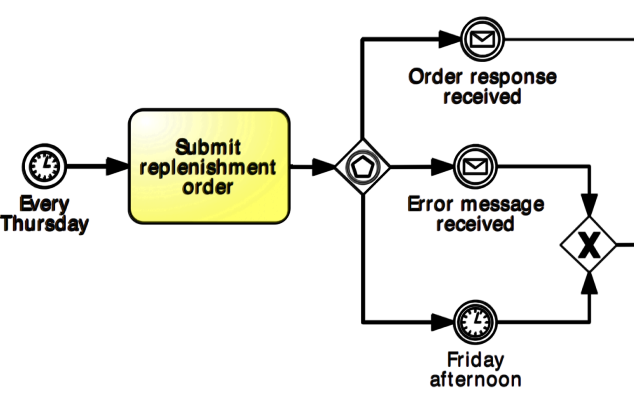
\includegraphics[width=0.6\textwidth]{images/bpmn/eventbasedexample.png}
    \caption{Example of Event-based Gateway in BPMN}
\end{figure}

\paragraph{Abortion:}
The simplest way to handle exceptions is to abort the process instance when an exception occurs.
This can be done via the Terminate End Event, which immediately ends the process instance regardless of its current state.
This causes the abortion of all ongoing activities and the termination of the process instance.
\begin{figure}[H]
    \centering
    
\includegraphics[width=0.2\textwidth]{images/bpmn/abortion.png}
    \caption{Abortion of a Process Instance in BPMN}
\end{figure}
We can use more sophisticated exception handling mechanisms, in order to recover from exceptions and continue the process flow.

\paragraph{Boundary Events}
Through boundary events, we catch intermediate events on the boundary of an activity or sub-process.
When the boundary event is triggered, the normal flow of the process is interrupted, and the exception handling flow is initiated.
There
\begin{itemize}
    \item \textbf{External boundary events}: triggered by events external to the process (handled with message events).
    \item \textbf{Internal boundary events}: triggered by events internal to the process (handled with error events).
    \begin{figure}[H]
        \centering
        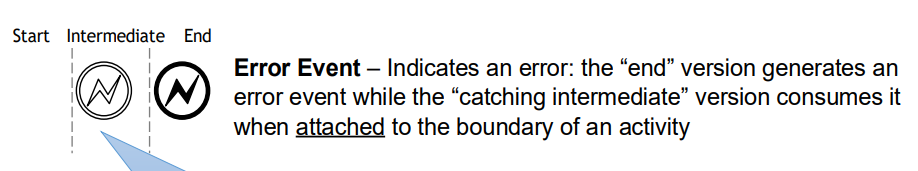
\includegraphics[width=0.8\textwidth]{images/bpmn/errorevent.png}
        \caption{Internal Boundary Event in BPMN}
    \end{figure}
    \item \textbf{Timeout boundary events}: triggered when a specified time duration elapses (handled with timer events).
    \begin{figure}[H]
        \centering
        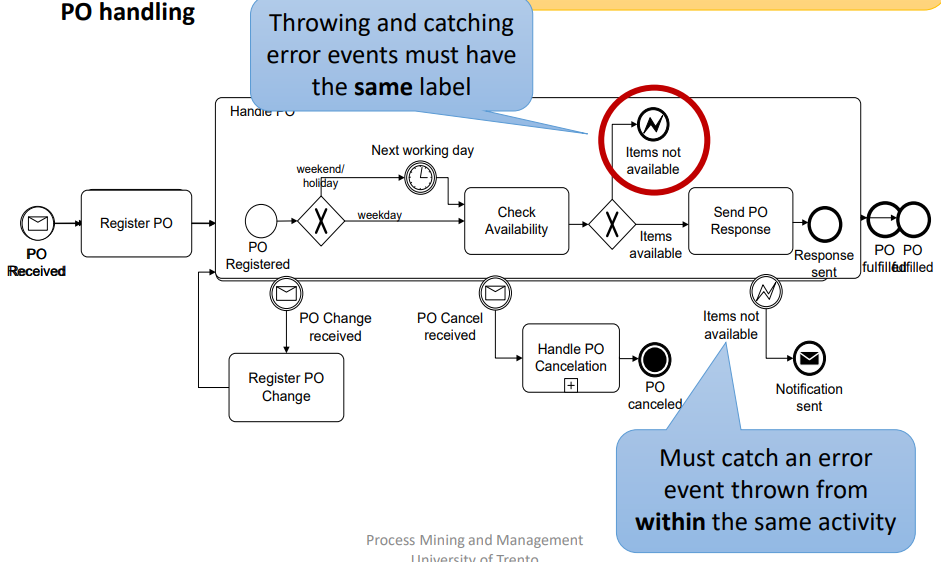
\includegraphics[width=0.8\textwidth]{images/bpmn/boundaryexample.png}
        \caption{Example of Boundary Events in BPMN}
    \end{figure}
\end{itemize}

\paragraph{Non-interrupting Boundary Events}
Sometimes, we want to handle exceptions without interrupting the normal flow of the process. In such cases, we can use non-interrupting boundary events.
When a non-interrupting boundary event is triggered, the exception handling flow is initiated, but the normal flow of the process continues concurrently.
\begin{figure}[H]
    \centering
    
\includegraphics[width=0.2\textwidth]{images/bpmn/non_interrupting.png}
    \caption{Non-interrupting Boundary Event in BPMN}
\end{figure}

\paragraph{Compensation Events}
Compensation events are used to handle situations where an activity needs to be undone or compensated for after it has been completed.
A compensation event is typically associated with a specific activity or sub-process, and it defines the actions that need to be taken to reverse or mitigate the effects of that activity.
\begin{figure}[H]
    \centering  
    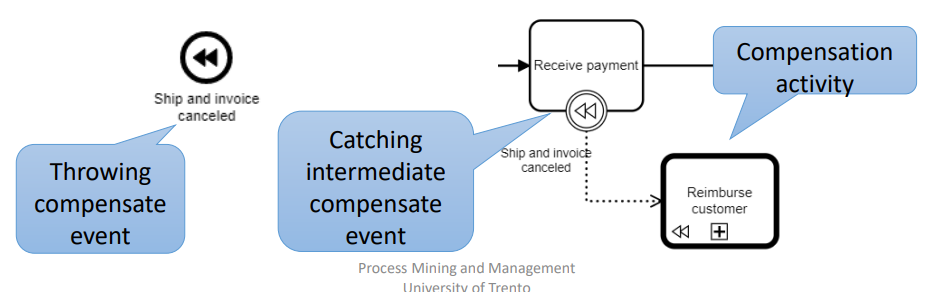
\includegraphics[width=0.6\textwidth]{images/bpmn/compensation.png}
    \caption{Compensation Event in BPMN}
\end{figure}

\subsection{Process Qualitative Analysis}

\subsubsection{Value-added analysis}
This kind of analysis focuses on \textbf{identifying and categorizing} activities within a business process based on their contribution to the overall value delivered to customers or stakeholders.
After that we can optimize the process by \textbf{eliminating} non-value-added activities.
\paragraph{Identification} We decorticate each activity in the process model and classify it into one of the following categories:
\begin{itemize}
    \item \textbf{Value-added activities}: directly contribute to meeting customer requirements 
        \begin{itemize}
            \item Is the customer willing to pay for this activity?
            \item Would the customer agree that this step is necessary to achieve their goals?
            \item If the step were eliminated, would the customer notice a difference in the final product or service?
        \end{itemize}
    \item \textbf{Business value-added activities}: necessary for the business but do not directly add value from the customer's perspective
        \begin{itemize}
            \item Is this step required in order to collect revenue, to improve or grow the business?
            \item Would the business pontentially suffer if this step were eliminated?
            \item Does it reduce risk of business losses?
            \item Is this step required to comply with regulations or legal requirements?
        \end{itemize}
    \item \textbf{Non-value-adding activities}: do not add value and are not necessary for the business (everything that is not VA or BVA)
\end{itemize}

\paragraph{Waste Elimination} After identifying and categorizing the activities, we can remove NVA activities and carefully evaluate BVA activities to see if they can be optimized or eliminated without negatively impacting the business.
We have different source of waste:
\begin{itemize}
    \item \textbf{Move}:
        \begin{itemize}
            \item \textbf{Transportation}: send or receive materials or document taken as input or output of an activity
            \item \textbf{Motion}: movement of resources internally within the process  
        \end{itemize}
    \item \textbf{Hold}:
        \begin{itemize}
            \item \textbf{Inventory}: accumulation of materials or documents waiting to be processed (Work in Progress - WIP)
            \item \textbf{Waiting}: task waiting for input data or resource availability, or resources waiting for task assignment
        \end{itemize}
    \item \textbf{Over-do}:
        \begin{itemize}
            \item \textbf{Defects}: correcting or compensating for errors or mistakes in the process (rework loops)
            \item \textbf{Over-processing}: tasks performed unnecessarily given the outcome required by the customer
            \item \textbf{Over-production}: unnecessary process instances are performed, producing outcomes that do not add value upon the completion of the process
        \end{itemize}
\end{itemize}

\subsection{Process Quantitative Analysis}
The process performance can be measured through different dimensions:
\begin{itemize}
    \item \textbf{Time}: how long it takes to complete a process or specific activities within the process
    \item \textbf{Cost}: the expenses incurred to execute the process, including labor, materials, and overhead costs
    \item \textbf{Quality}: the degree to which the process meets customer requirements and expectations
\end{itemize}

\subsubsection*{Time Measures}

\paragraph{Cycle (throughput) time}: the time between start and completion of a process instance.
It can be measured as:
\begin{equation}
    \text{Cycle throughput time} = \text{Processing Time (PT)} + \text{Waiting Time (WT)}
\end{equation}
where:
\begin{itemize}
    \item \textbf{Processing Time (PT)}: time taken by value-adding activities
    \item  \textbf{Waiting Time (WT)}: time spent in non-value-adding activities
\end{itemize}

The result can be different from a simply sum, depending on the process structure (e.g., parallel paths, loops, etc.).
\begin{figure}[H]
    \centering
    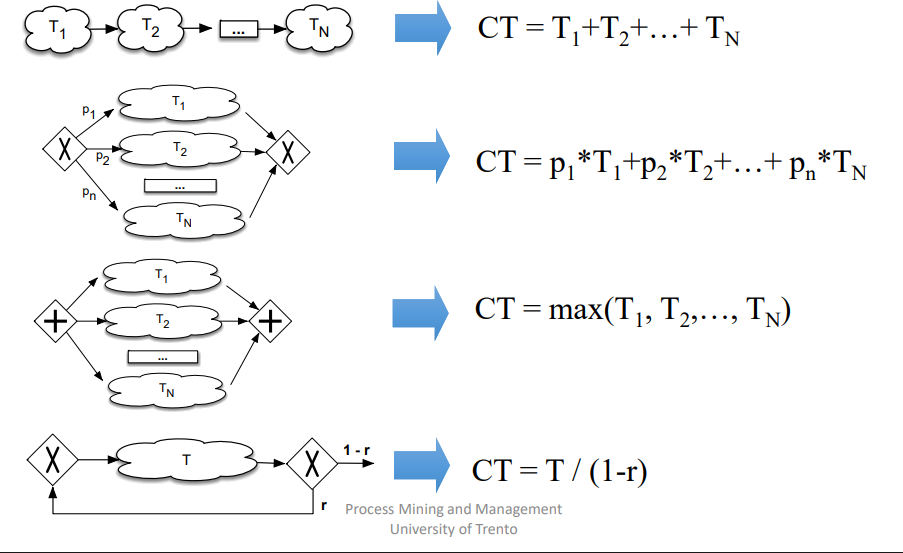
\includegraphics[width=0.9\textwidth]{images/bpmn_analysis/CTE_table.png}
    \caption{Cycle Time Calculation Table}
\end{figure}

\paragraph{Cycle Time Efficiency}
The Cycle Time Efficiency (CTE) is a measure of how efficiently a process is executed, focusing on the proportion of time spent on value-adding activities compared to the total cycle time.
It is calculated as:
\begin{equation}
    \text{CTE} = \frac{\text{Processing Time (PT)}}{\text{Cycle throughput time}} 
\end{equation}

\paragraph{Per-instance Cost}
The per-instance cost of a process measures the total cost incurred to complete a single instance of the process.
It is calculated as:
\begin{equation}
    \text{Per-instance Cost} = \text{Processing cost} + \text{Cost of waste}
\end{equation}
where:
\begin{itemize}
    \item \textbf{Processing cost}: cost associated with value-adding activities
    \item  \textbf{Cost of waste}: cost associated with non-value-adding activities
\end{itemize}

\subsubsection*{Quality}

\paragraph{Work-In-Progress (WIP)}
It's the number of cases that are running, but they are not yet completed.
WIP is a form of waste. 
Can be calculated as:
\begin{equation}
    \text{WIP} = \lambda \times \text{Cycle Time}
\end{equation}
where $\lambda$ is the arrival rate (number of cases arriving per time unit).
Its limitation is that we can't estimate waiting times or queue lengths.